\subsection{Mikrocontroller} \label{sec:microcontrollerHardware}
Für die Steuerung der Anwendung wird nun noch ein zentraler Controller benötigt. Die Wahl fiel auf den Mikrocontroller nRF52832 von Nordic Semiconductors. Seine hohe Performance ermöglicht es ein System aufzubauen, welches nur eine zentrale Schnittstelle beinhaltet. Abbildung \ref{fig:nRF52832} zeigt den Controller als Einzelbauteil und als Entwicklungskit-Kit.


\begin{figure}[H]
	\centering
	\subfigure[nRF52832 Microcontroller \cite{nRF52832}]{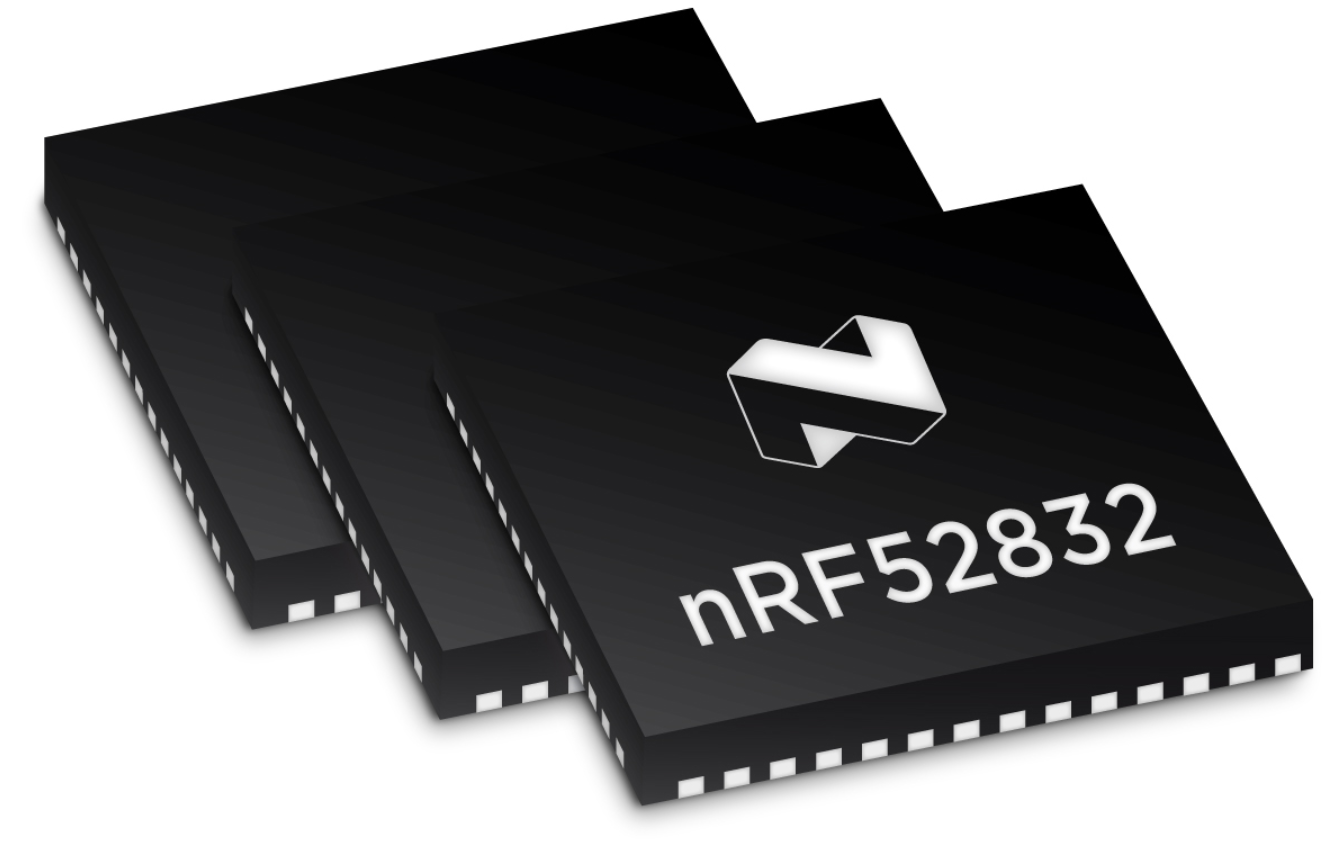
\includegraphics[width = 0.45\textwidth]{data/nRF52832.png}}\quad
	\subfigure[nRF52 Development Kit \cite{nRF52-DK}]{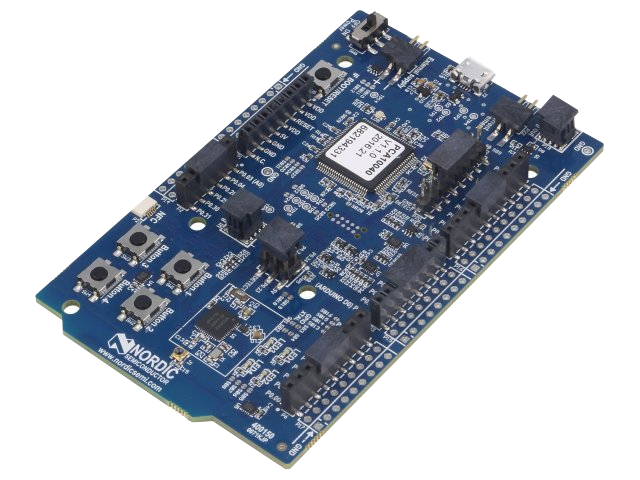
\includegraphics[width = 0.45\textwidth]{data/NRF52-DK.png}}\quad
	\caption[Mikrocontroller NRF52832]{Mikrocontroller als Einzelelement und als Entwicklungsanwendung}
	\label{fig:nRF52832}
\end{figure}

Der nRF52832 weist eine Betriebsversorgungsspannung zwischen 1.7V und 3.6V mit einem Versorgungsstrom von 5.4mA auf. Diese niedrigen Werte ermöglichen einen dauerhaften Betrieb durch die integrierte Batterie. Die Speicherkapazität ist durch 512kB flash/64kB RAM Speicher gegeben. Für die Entwicklung des Prototypen wurde das Entwicklungsboard verwendet. Dies hat verschiedene Vorteile, wie z.B. die integrierte Bluetooth-Antenne, die einfache Verwendung von sogenannten Shields und das einfache Handling für Messungen und provisorische Verbindungen.